\documentclass[11pt]{beamer}
\usetheme{CambridgeUS}
\usecolortheme{dolphin}

\usepackage[utf8]{inputenc}
\usepackage[brazil]{babel}
\usepackage[T1]{fontenc}
\usepackage{xcolor}
\usepackage{amsmath}
\usepackage{amsfonts}
\usepackage{amssymb}
\usepackage{graphicx}
\usepackage{setspace}
\usepackage{ragged2e}

\setbeamertemplate{caption}[numbered]

% Controle do gabarito %
%%%%%%%%%%%%%%%%%%%%%
\newif\ifgab
\gabtrue
\newcommand{\gab}[1]{%
  \ifgab
    \textcolor{red!80!black}{\textbf{#1}}%
  \else
    #1%
  \fi
}
%%%%%%%%%%%%%%%%%%%%%

\author[CETi / IFAM CMC]{Autores \\ Professores: Luiz Claudio e Joao Victor}
\title{Função Quadrática - (UEA/ENEM)}
%\setbeamercovered{transparent} 
\setbeamertemplate{navigation symbols}{} 
\institute[]{CETi BILÍNGUE GILBERTO MESTRINHO \par INSTITUTO FEDERAL DO AMAZONAS } 
\date{\today} 
\titlegraphic{
\includegraphics[width=0.6\textwidth]{imagens/logo.png}}

%\subject{}

% ---------------------------------------------------------

\begin{document}
\justifying
\onehalfspacing 

\begin{frame}
    \titlepage
\end{frame}

\section{Função Quadrática}

\section{Teoria}

\begin{frame}{Teoria}

    \begin{block}{\textbf{Definição}}
        Dados os números reais $a, b$ e $c$, $a \neq 0$, a função $f: \mathbb{R} \to \mathbb{R}$ definida por $f(x)=ax^{2}+bx+c$, $\forall \ x \in \mathbb{R}$, é denominada \textbf{função polinomial do 2º grau (ou função quadrática)}
    \end{block}

    \pause 
    
    \begin{block}{\textbf{Gráfico}}
        O gráfico de uma função quadrática é uma curva aberta denominada \textbf{parábola}, com \textit{eixo de simetria} paralelo ao \textit{eixo das ordenadas}
    \end{block}
    
\end{frame}

\begin{frame}{Teoria}

    \begin{block}{\textbf{Raízes e estudo de sinais}}
        Dada a função $f: \mathbb{R} \to \mathbb{R}$ definida por $f(x)=ax^{2}+bx+c, a \neq 0, \forall \ x \in \mathbb{R}$ determinamos duas raízes (ou zeros) fazendo $f(x)=0$. Temos, então $ax^{2}+bx+c=0$, onde: $x=-\dfrac{b\  \pm \ \sqrt{\Delta}}{2a}$, e $\Delta=b^{2}-4ac$.
    \end{block}

    \pause 
    
    \begin{block}{Estudo do discriminante}
        \begin{enumerate}[I]
            \item $\Delta > 0 \Rightarrow f$ tem duas raízes reais e distintas.
            \item $\Delta = 0 \Rightarrow f$ tem duas raízes reais e iguais.
            \item $\Delta < 0 \Rightarrow f$ não tem raízes reais.
        \end{enumerate}
        
    \end{block}
    
\end{frame}

\begin{frame}{Teoria}

    \begin{block}{\textbf{Vértice e concavidade}}
        O ponto $V(X_{v}, Y_{v})$ é denominado vértice da parábola. Suas coordenadas são dadas por: $X_{v}=-\dfrac{b}{2a}$ e $Y_{v}=-\dfrac{\Delta}{4a} \Rightarrow  V \left ( -\dfrac{b}{2a}, -\dfrac{\Delta}{4a} \right )$. \textit{Dica: temos ainda que $Y_{v}=f(X_{v})$}
    \end{block}

    \pause 
    
    \begin{block}{}
        Na função $f(x)=ax^{2}+bx+c$, temos:

        \begin{enumerate}[I]
            \item $a > 0$: Parábola com concavidade voltada para cima.
            \item $a < 0$: Parábola com concavidade voltada para baixo.
        \end{enumerate}
    \end{block}
    
\end{frame}

\begin{frame}{Teoria - Vértice e concavidade (continuação)}

    \begin{block}{Para $a>0$, temos:}
        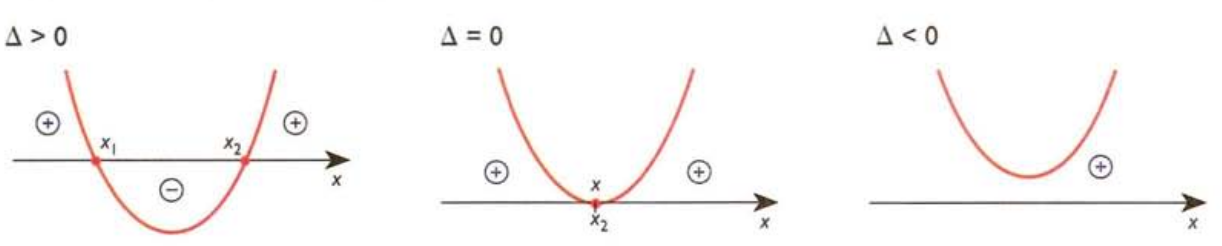
\includegraphics[scale=0.27]{imagens/func1.png}
    \end{block}

    \pause
    
    \begin{block}{Para $a<0$, temos:}
        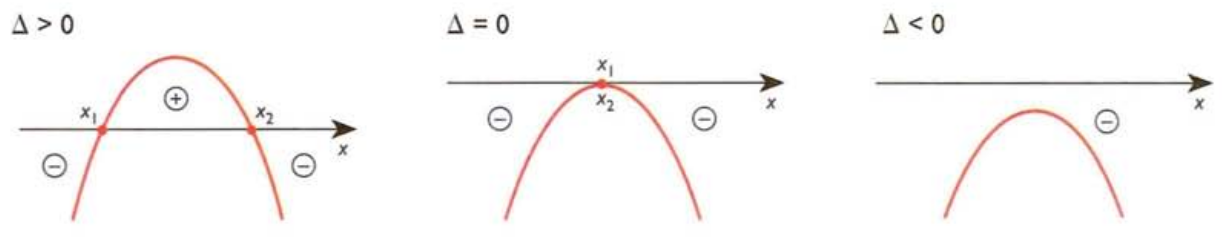
\includegraphics[scale=0.27]{imagens/func2.png}
    \end{block}
\end{frame}

\begin{frame}{Teoria}

    \begin{block}{\textbf{Outras formas para $f(x)$}}
        Sendo $x_{1}$ e $x_{2}$ raízes de $f(x)$, temos que $f(x)=ax^{2}+bx+c$ pode ser reescrita como $f(x)=a(x-x_{1})(x-x_ {2})$
    \end{block}

    \pause 
    
    \begin{block}{Forma canônica}
        Podemos reescrever $f(x)=ax^{2}+bx+c$ em função das coordenadas do vértice: $X_{v}$ e $Y_{v}$, da seguinte forma: $f(x)=a(x-X_{v})^{2}+Y_{v}$
    \end{block}
    
\end{frame}



\section{Questões}

\begin{frame}{ENEM 2013}
    
    A parte interior de uma taça foi gerada pela rotação de uma parábola em torno de um eixo z, conforme mostra a figura. A função real que expressa a parábola, no plano cartesiano da figura, é dada pela lei: $f(x)=\dfrac{3}{2}x^{2}-6x+c$ onde C é a medida da altura do líquido contido na taça, em centímetros. Sabe-se que o ponto V, na figura, representa o vértice da parábola, localizado sobre o eixo x. 

    \vfill
    \textbf{(continua no próximo slide)}
    
\end{frame}

\begin{frame}{ENEM 2013 (continuação)}
    Nessas condições, a altura do líquido contido na taça, em centímetros, é:
    \begin{columns}
        \begin{column}{0.4\textwidth}
            \begin{enumerate}[a]
                \item $1$ 
                \item $2$  
                \item $4$
                \item $5$ 
                \item \gab{$6$} %
            \end{enumerate}
        \end{column}

        \begin{column}{0.6\textwidth}
            \centering
            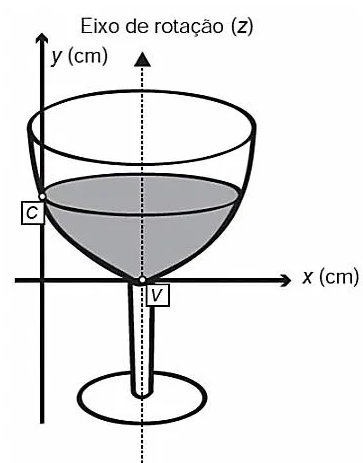
\includegraphics[width=0.7\linewidth]{imagens/enem 2013.png}
        \end{column}
    \end{columns}
    
\end{frame}

\begin{frame}{ENEM 2014}

    Um professor, depois de corrigir as provas de sua turma, percebeu que várias questões estavam muito difíceis. Para compensar, decidiu utilizar uma função polinomial f, de grau menor que 3, para alterar as notas x da prova para notas $y = f(x)$, da seguinte maneira:

    \begin{enumerate}[I]
        \item A nota zero permanece zero.
        \item A nota 10 permanece 10.
        \item A nota 5 passa a ser 6.
    \end{enumerate}

    \vfill
    \textbf{(continua no próximo slide)}
    
\end{frame}

\begin{frame}{ENEM 2014 (continuação)}
    A expressão da função $y = f(x)$ a ser utilizada pelo professor é:

    \begin{enumerate}[a]
        \item \gab{$y=-\dfrac{1}{25}x^{2}+\dfrac{7}{5}x$} % \\
        \item $y=-\dfrac{1}{10}x^{2}+2x$ \\
        \item $y=\dfrac{1}{24}x^{2}+\dfrac{7}{12}x$ \\
        \item $y=\dfrac{4}{5}x+2$ \\
        \item $y=x$ 
    \end{enumerate}
    
\end{frame}

\begin{frame}{ENEM PPL 2019}
    No desenvolvimento de um novo remédio, pesquisadores monitoram a quantidade Q de uma substância circulando na corrente sanguínea de um paciente, ao longo do tempo t. Esses pesquisadores controlam o processo, observando que Q é uma função quadrática de t. Os dados coletados nas duas primeiras horas foram:

    \begin{center}
        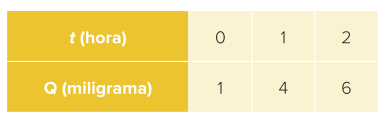
\includegraphics[scale=0.5]{imagens/enem-ppl-2019.png}
    \end{center} \textbf{(continua no próximo slide)}
\end{frame}

\begin{frame}{ENEM PPL 2019 (continuação)}
    Para decidir se devem interromper o processo, evitando riscos ao paciente, os pesquisadores querem saber, antecipadamente, a quantidade da substância que estará circulando na corrente sanguínea desse paciente após uma hora do último dado coletado. Nas condições expostas, essa quantidade (em miligrama) será igual a:

    \begin{enumerate}[a]
        \item $4$
        \item \gab{$7$} %
        \item $8$ 
        \item $9$ 
        \item $10$ 
    \end{enumerate}
\end{frame}

\begin{frame}{ENEM 2022}

    Ao analisar os dados de uma epidemia em uma cidade, peritos obtiveram um modelo que avalia a quantidade de pessoas infectadas a cada mês, ao longo de um ano. O modelo é dado por $p(t)=-t^{2}+10t+24$, sendo t um número natural, variando de 1 a 12, que representa os meses do ano, e p(t) a quantidade de pessoas infectadas no mês t do ano. Para tentar diminuir o número de infectados no próximo ano, a Secretaria Municipal de Saúde decidiu intensificar a propaganda oficial sobre os cuidados com a epidemia. Foram apresentadas cinco propostas (I, II, III, IV e V), com diferentes períodos de intensificação das propagandas: $\textbf{(I)}\ 1 \leq t \leq 2, \textbf{(II)}\ 3 \leq t \leq 4, \textbf{(III)}\ 5 \leq t \leq 6, \textbf{(IV)}\ 7 \leq t \leq 9$ e $\textbf{(V)}\ 10 \leq t \leq 12$

    \vfill
    \textbf{(continua no próximo slide)}
\end{frame}
\begin{frame}{ENEM 2022 (continuação)}
    A sugestão dos peritos é que seja escolhida a proposta cujo período de intensificação da propaganda englobe o mês em que, segundo o modelo, há a maior quantidade de infectados. A sugestão foi aceita. A proposta escolhida foi a:

    \begin{enumerate}[a]
            \item I
            \item II
            \item \gab{III} %
            \item IV 
            \item V
        \end{enumerate}
\end{frame}

\begin{frame}{UEA - 2014}

    Em um sistema de coordenadas cartesianas ortogonais, os gráficos das funções quadráticas $f(x) = -2x^{2} + 5x + 3$ e $g(x)$ são simétricos um do outro com relação ao eixo das abscissas. Desse modo, é correto afirmar que a distância entre os seus vértices é igual a:

    \begin{enumerate}[a]
        \item 12,05
        \item 6,25
        \item 8,15
        \item 6,12
        \item \gab{12,25} %
    \end{enumerate}
    
\end{frame}

\begin{frame}{UEA - 2015}
    Considere o gráfico da função quadrática dada por $f(x) = -x^{2} + 2x + c$. De acordo com o gráfico, é correto afirmar que o valor de y é:
    \begin{columns}
        \begin{column}{0.4\textwidth}
            \begin{enumerate}[a]
                \item negativo, se $x < 3$
                \item positivo, se $x > 3$
                \item \gab{positivo, no intervalo $ -1 < x < 3$} %
                \item negativo, se $x > -1$
                \item zero, se $x = 1$
            \end{enumerate}
        \end{column}

        \begin{column}{0.6\textwidth}
            \centering
            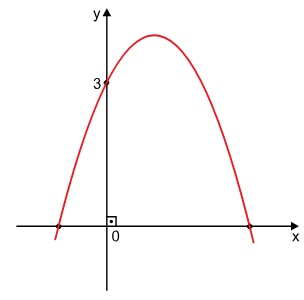
\includegraphics[width=0.7\linewidth]{imagens/uea-2015.png}
        \end{column}
    \end{columns}
    
\end{frame}

\begin{frame}{UEA - 2017}
    O gráfico da função real $f(x)=ax^{2}+ bx + c$, com $a > 0$, é a parábola representada na figura. Sabendo-se que $x_{1}+x_{2}= -{b}/2$, onde $ x_{1}, x_ {2}$ são as raízes de $f(x) = 0$, é correto afirmar que a parábola intersecta o eixo das ordenadas no ponto:

    \begin{columns}
        \begin{column}{0.4\textwidth}
            \begin{enumerate}[a]
                \item $(0,12)$ 
                \item $(12,0)$
                \item $(0,4)$ 
                \item \gab{$(0,16)$} %
                \item $(16,0)$
            \end{enumerate}
        \end{column}

        \begin{column}{0.5\textwidth}
            \centering
            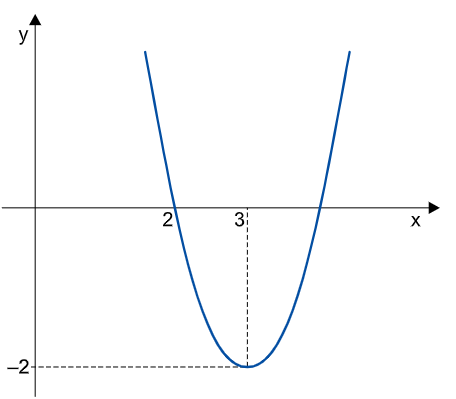
\includegraphics[width=0.8\linewidth]{imagens/uea-macro-2017(2).png}
        \end{column}
    \end{columns}
    
\end{frame}

\begin{frame}{Vunesp}
    Uma função quadrática tem o eixo dos y como eixo de simetria. A distância entre os zeros da função é de 4 unidades, e a função tem $-5$ como valor mínimo. Esta função quadrática é:

    \begin{enumerate}[a]
        \item $y=5x^{2}-4x-5$
        \item $y=5x^{2}-20$ \\
        \item $y=\dfrac{5}{4}x^{2}-5x$ \\
        \item \gab{$y=\dfrac{5}{4}x^{2}-5$} \\ %
        \item $y=\dfrac{5}{4}x^{2}-20$
    \end{enumerate}
\end{frame}

\begin{frame}{IFPE 2019}
    Um balão de ar quente sai do solo às 9h da manhã (origem do sistema cartesiano) e retorna ao solo 8 horas após sua saída, conforme demons- trado a seguir. A altura h, em metros, do balão, está em função do tempo t, em horas, através da fórmula $h(t)=(-{3}/{4})t^{2}+6t$ .

    \begin{center}
        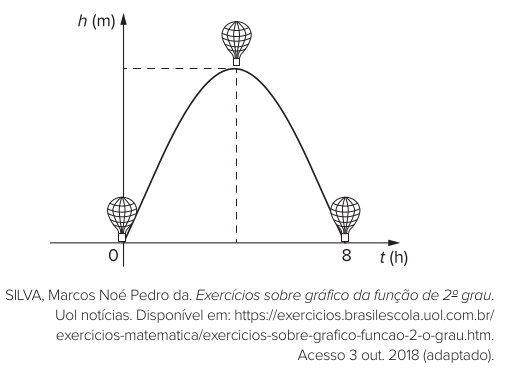
\includegraphics[scale=0.5]{imagens/IFPE 2019.png}
    \end{center}
\end{frame}

\begin{frame}{IFPE 2019 (continuação)}
    A altura máxima atingida pelo balão é de:

    \begin{enumerate}[a]
        \item 21 m 
        \item 36 m
        \item 8 m 
        \item 4 m
        \item \gab{12 m} %
    \end{enumerate}
\end{frame}

\begin{frame}{AFA}
    Para que o valor mínimo da função $y=x^{2}-4x+k$ seja igual a $-1$, o valor de k é:

    \begin{enumerate}[a]
        \item 1
        \item 2
        \item \gab{3} %
        \item 4
        \item 5
    \end{enumerate}
\end{frame}

\begin{frame}{PUC - Campinas SP - 2015}
    A figura indica um bombeiro lançando um jato de água para apagar o fogo em um ponto de uma torre retilínea e perpendicular ao chão. A trajetória do jato de água é parabólica, e dada pela função $y = -x^{2} + 2x + 3$ , com x e y em metros. Sabendo que o ponto de fogo atingido pelo jato de água está a 2 metros do chão, então, qual o valor de $p-q$, em metros?

    \begin{columns}
        \begin{column}{0.4\textwidth}
            \begin{enumerate}[a]
                \item $2+\sqrt{2}$ 
                \item $1+\sqrt{2}$  
                \item $4-2\sqrt{2}$
                \item $3-\sqrt{2}$ 
                \item \gab{$2-\sqrt{2}$} %
            \end{enumerate}
        \end{column}

        \begin{column}{0.6\textwidth}
            \centering
            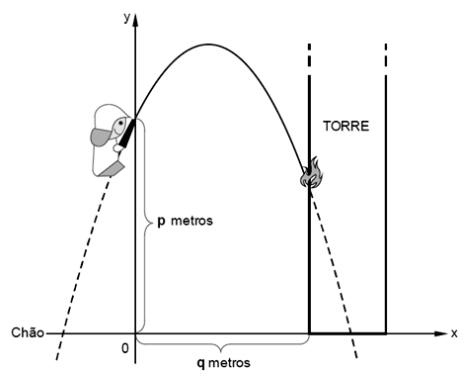
\includegraphics[width=0.75\linewidth]{imagens/q20.png}
        \end{column}
    \end{columns}
\end{frame}

\begin{frame}{Unifor-CE}
    Na figura abaixo têm-se os gráficos das funções quadráticas f e g. Se P é um dos pontos de interseção de f e g, então as suas coordenadas são:

    \begin{columns}
        \begin{column}{0.4\textwidth}
            \begin{enumerate}[a]
                \item $(-{3}/{4},{57}/{16})$ 
                \item \gab{$(-{1}/{2},{9}/{4})$}  %
                \item $(-{1}/{2},-{9}/{4})$
                \item $(-{1}/{4},{17}/{16})$ 
                \item $(-{1}/{4},-{17}/{16})$
            \end{enumerate}
        \end{column}

        \begin{column}{0.6\textwidth}
            \centering
            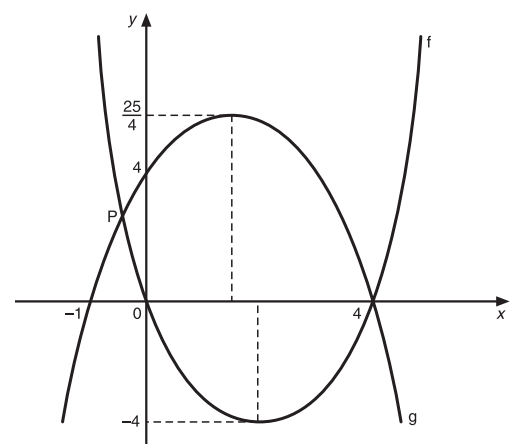
\includegraphics[width=0.9\linewidth]{imagens/Unifor-CE.png}
        \end{column}
    \end{columns}
    
\end{frame}

\end{document}
